%!TEX root = ../thesis.tex

% \pagebreak[4]
% \hspace*{1cm}
% \pagebreak[4]
% \hspace*{1cm}
% \pagebreak[4]

\chapter{Mélange d'outils}

\graphicspath{ {Chapter3/Chapter3Figs/PNG/}
  {Chapter3/Chapter3Figs/PDF/} {Chapter3/Chapter3Figs/} }

Nous avons vu que les outils de déformation avaient différentes
caractéristiques. Celles-ci influent sur l'aspect de la déformation engendrée
par le déplacement de points de contrôle, ainsi que sur la facilité de
déformation du modèle. Une modification grossière de l'apparence globale de le
modèle est plus facile à réaliser avec un outil de déformation gloable ayant
une faible résolution. A l'inverse, la modification d'un ensemble de points
précis du modèle nécessite l'utilisation d'un outil de déformation locale et
une résolution élevée. Il est naturel de se demander alors comment combiner
différents outils associé à un même modèle, de façon à ce que la déformation
soit visuellement lisse.

\section{Etat de l'art}

\cite{JBPS11} sont les premiers à proposer une méthode permettant de mélanger
des outils de déformation de différentes dimensions. C'est sur cet article que
nous avons commencé à travailler car les résultats nous semblaient proches de
ce que nous souhaitons réaliser. Une lecture approfondie de l'article nous a
fait comprendre que la méthode n'était pas celle que nous souhaitions. Même si
l'article semble s'appuyer sur des outils ayant des dimensions différentes en
fonction des zones à déformer, la gestion interne repose uniquement sur des
déformations à base de points. Des contraintes supplémentaires sont imposées
lors du calcul des coordonnées en fonction de la topologie existante entre les
points de contrôle. Par exemple pour des sommets reliés par une arête les
auteurs proposent que les coordonnées évoluent de façon linéaire le long de
cette arête. De plus, pour évaluer l'influence d'un point de contrôle sur
l'espace, la technique proposée se base sur une méthode de diffusion
(nécessitant donc une discrétisation de l'espace). Or un des critères
essentiels de notre travail est la minimisation des temps de calcul, c'est
pourquoi nous avons décidé de pas continuer à étudier cette technique et à
nous intéresser à un autre travail du domaine.

\cite{GPCP13} quant à eux, proposent une méthode permettant le mélange
d'outils de même dimension, en s'intéressant particulièrement aux cas des
déformations à base de cage. L'idée est de réaliser un pavage de différentes
cages sur tout l'espace à déformer  collées ensemble le long de leurs arêtes
et de considérer la position d'un point de l'espace, et pas seulement par
rapport à sa cage \textit{propre} (à comprendre la cage englobant le point de
l'espace) mais aussi par rapport aux cages adjacentes à celle-ci. Cette
technique permet de localiser la déformation engendrée par un sommet d'une
cage sur la zone couverte par sa cage propre et l'ensemble des cages
incidentes à celle-ci. Cette méthode impose de placer des cages sur l'ensemble
du modèle, sans présumer de la déformation qui est à appliquer. Les cages
créées doivent être collées le long de leurs arêtes pour que la méthode
fonctionne, et cette contrainte alourdit les traitements à effectuer, du fait
des nombreux cas spécifiques que la méthode doit traiter. En particulier,
cette méthode repose en interne sur une discrétisation de l'espace par
l'utilisation de coordonnées harmoniques, ce qui est incompatible avec la
minimisation du temps de calcul qui est une de nos priorités.

Comme les solutions existantes ne correspondent pas exactement à ce que nous
souhaitons, nous avons décidé de travailler sur une autre approche afin
d'apporter une contribution originale au niveau des mélanges d'outils de
déformations.

\section{Méthode proposée}

Nous nous sommes concentrés sur des déformations à base de cage, certaines
idées de \cite{GPCP13} nous ont semblé intéressantes, et nous avons décidé de
nous en inspirer. Notre contribution est double :

\begin{enumerate}

\item Modifier la zone d'influence des déformations à base de cages

\item Combiner les effets des déformations appliquées par les différentes
cages

\end{enumerate}

\subsection{Modification de la zone d'influence des déformations}

Pour d'apporter plus d'explications quant à l'origine de nos contributions,
nous illustrons les problèmes qui peuvent se produire lorsqu'un modèle n'est
qu'inclus partiellement dans une cage.

En calculant uniquement des coordonnées pour les points de l'espace à
l'intérieur de la cage et en ne tenant pas compte des points à l'extérieur de
celle-ci, les problèmes se traduisent par une brusque transition entre
l'intérieur et l'extérieur de la cage (Figure \ref{MELVI}). Visuellement la
déformation n'est pas lisse.

\begin{figure}[ht]
  \begin{center}
    \scalebox{0.2}
    {
      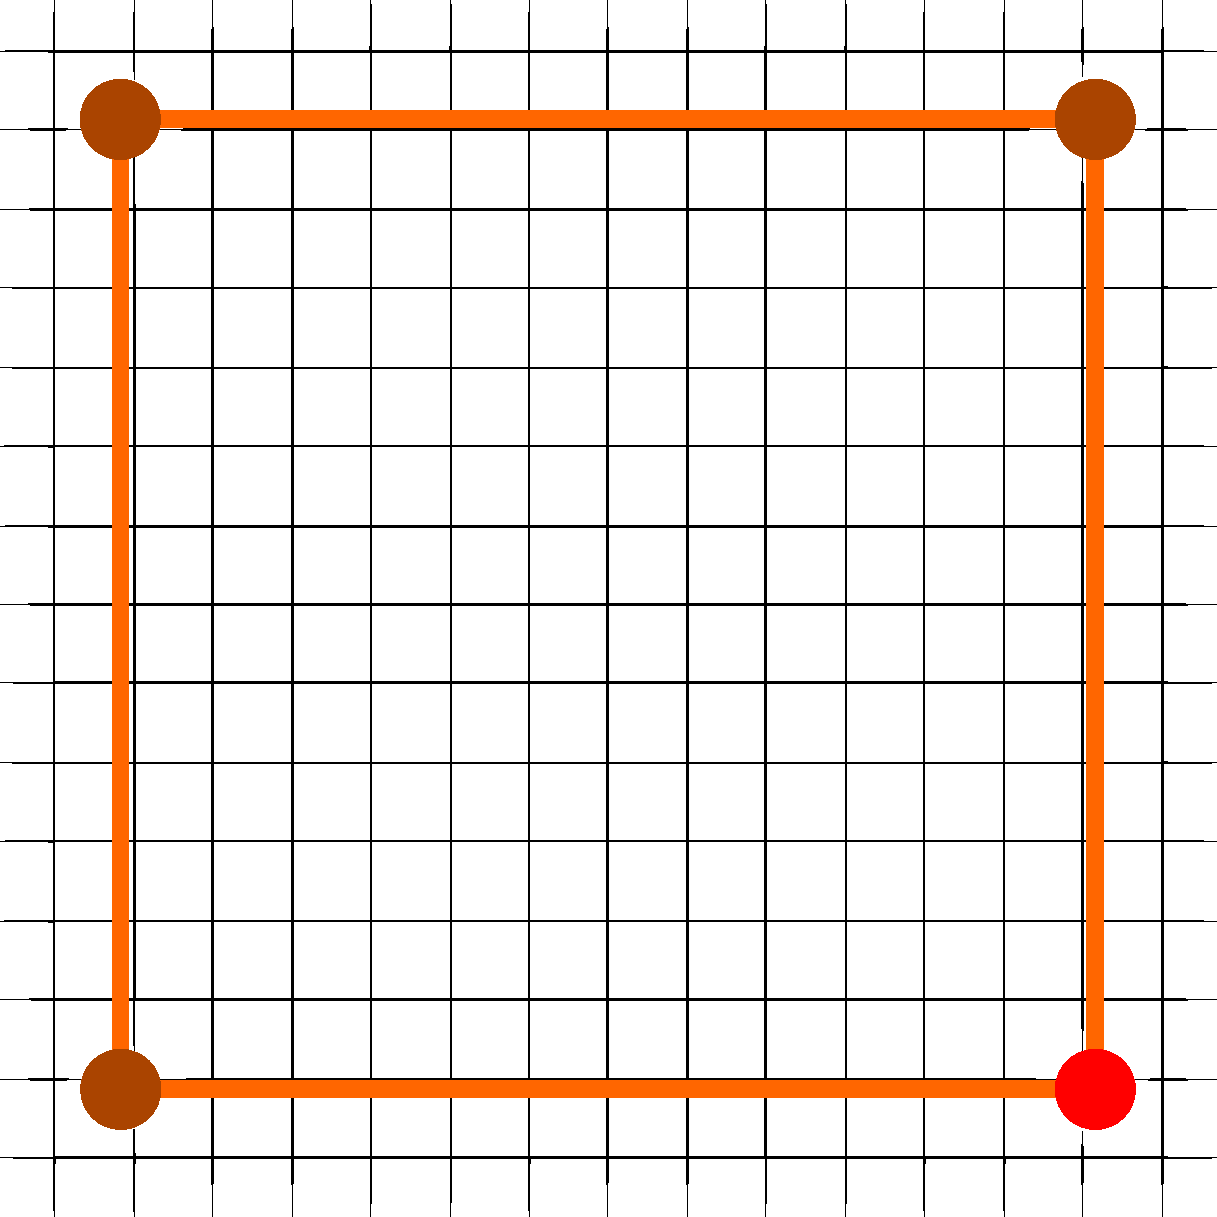
\includegraphics{Deformation-Interieur-1Sommet-Avant}
      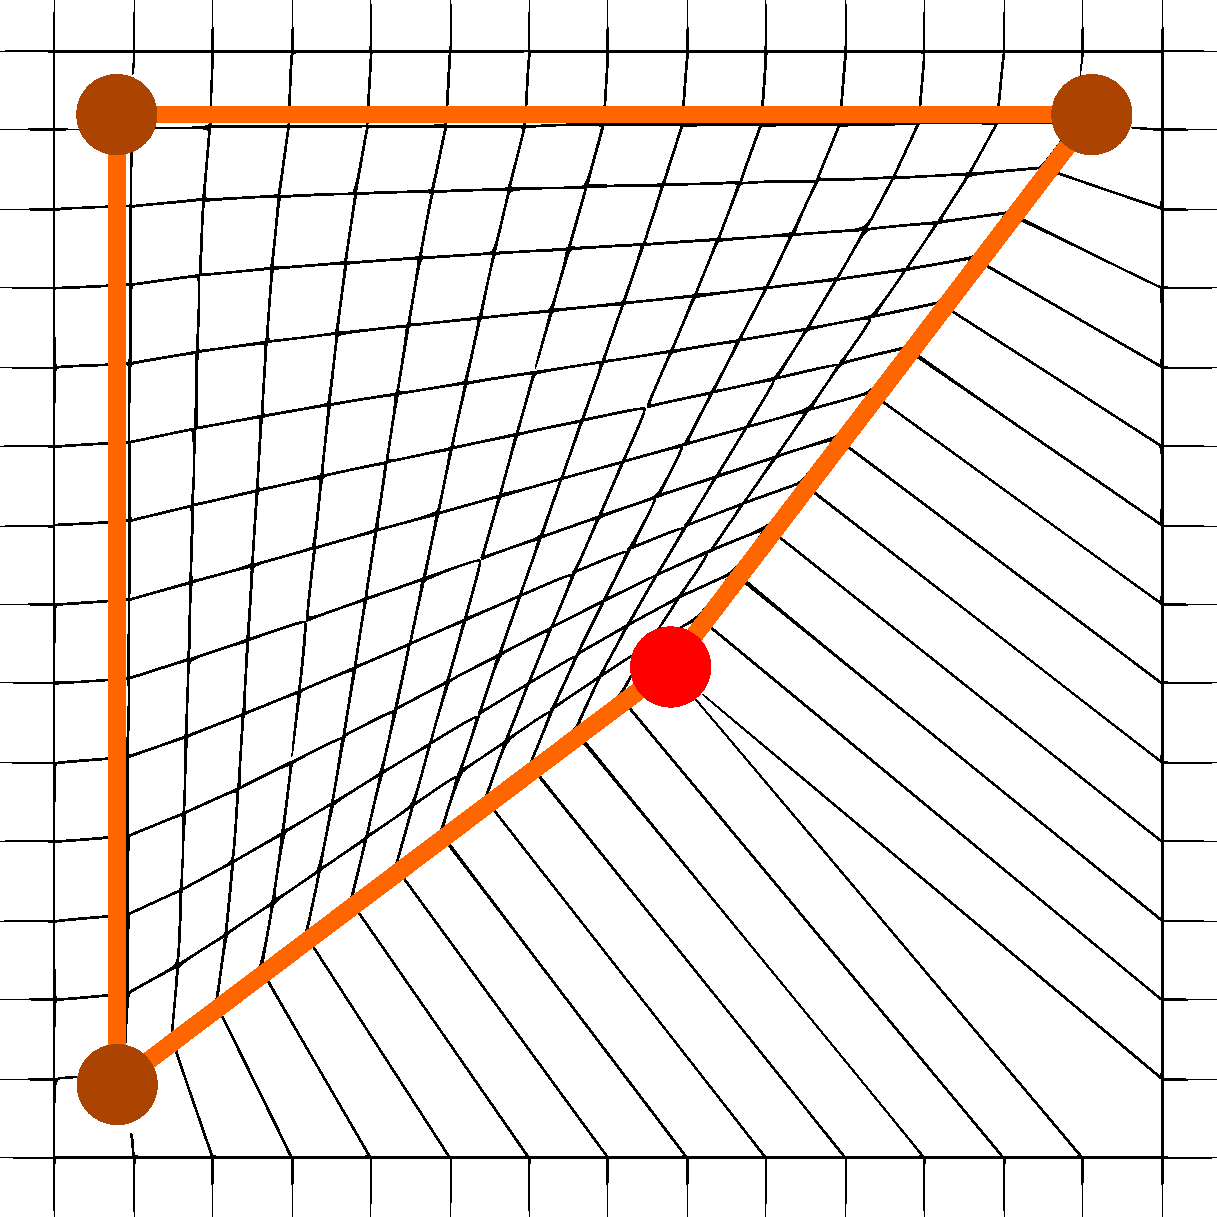
\includegraphics{Deformation-Interieur-1Sommet-Apres}
    }

    \caption[Problème de continuité déformation naïve] {Visualisation des
problèmes de continuité lorsque seuls les points à l'intérieur sont déformés.
Le bord de la cage est représenté en bleu. Le sommet en rouge représente le
sommet déplacé. A gauche le modèle avant déformation, à droite le même modèle
après déformation.}

    \label{MELVI}
  \end{center}
\end{figure}

En considérant des coordonnées pour les points de l'espace à la fois à
l'intérieur et à l'extérieur de la cage le problème vient de la dérivabilité
de la fonction résultant de la déformation. Plus précisément, pour les MVC et
GC la fonction de déformation est définie dans $\mathbb{R}^2$ et est
$C^{\infty}$ partout sauf au niveau des sommets de la cage où elle n'est que
$C^0$ (d'après \cite{LS08}). La déformation engendrée n'est pas visuellement lisse autour des
sommets de la cage. Quant aux HC, elles ne sont définies qu'à l'intérieur de
la cage où elles sont $C^{\infty}$, il n'y a donc aucun moyen de déformer
l'extérieur de la cage de cette manière.

Notre objectif est d'obtenir une fonction de déformation, définie par une
cage, qui soit au moins $C^1$ partout (visuellement lisse) et dont la zone
d'influence soit limitée.

Plutôt que de mettre en place une nouvelle méthode de calcul de coordonnées
ayant les propriétés que nous souhaitons nous nous intéressons plutôt à la
réutilisation des méthodes de calcul existantes afin d'exploiter leur qualités.

\subsubsection{Principe}

Nous considérons deux cages là où les travaux antérieurs n'en considéraient
qu'une seule. Nous appelons \textit{cage de contrôle} la cage avec laquelle
l'utilisateur interagit pour réaliser les déformations. Nous appelons
\textit{cage d'influence} la cage qui définit la zone d'influence (points de
l'espace qui sont sous l'influence de la déformation). La cage d'influence est
homothétique à la cage de contrôle et contient strictement cette dernière
(Figure \ref{MELDou}).

\begin{figure}[ht]
  \begin{center}
    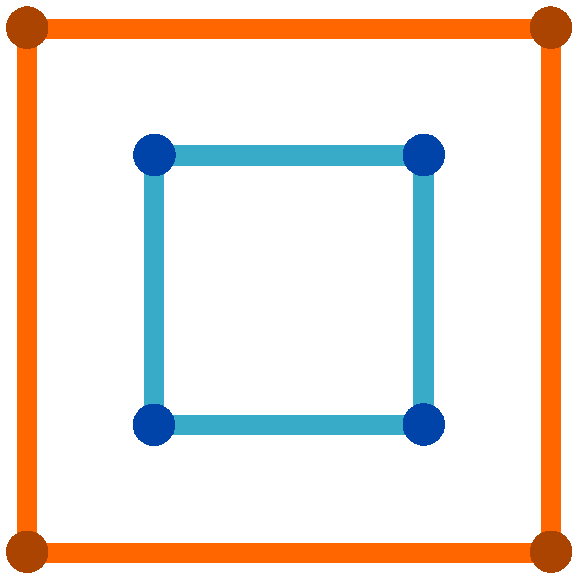
\includegraphics[scale=0.5]{chapter3-doubleCage-pstricks}

    \caption[Disposition des cages de contrôle et d'influence] {Disposition
des deux cages. En bleu la cage de contrôle, en orange la cage d'influence.}

    \label{MELDou}
  \end{center}
\end{figure}

Avec cette disposition, l'extérieur de la cage de contrôle peut-être
interprêté comme l'intérieur de la cage d'influence. Il se trouve que les
coordonnées MVC sont $C^{\infty}$ à l'intérieur de la cage d'influence (par
définition), les déformations qui ont lieu à l'intérieur de celle-ci sont donc
visuellement lisses. On introduit une notion de hiérarchie de déformation, où
la modification de la position des sommets de la cage de contrôle va modifier
la position des sommets de la cage d'influence, qui elle- même va modifier
l'espace contenu en son intérieur, grâce aux méthodes de calcul de coordonnées
existantes (MVC, HC, GC). \\

\subsubsection{Hiérarchie de la déformation}

Il faut maintenant établir un lien entre les deux cages, afin que la
modification de la position des sommets de la cage de contrôle affecte la
position des sommets de la cage d'influence.

Une première idée est d'utiliser des coordonnées barycentriques généralisées
pour définir la position de chacun des sommets de la cage d'influence comme
une combinaison linéaire pondérée des positions des sommets de la cage de
contrôle. Cette technique pose un problème quant à la localité de la
déformation. Même si la déformation s'effectue dans toute la zone d'influence,
on souhaite que les points les plus éloignés du sommet modifié soient le moins
affectés par la déformation engendrée.

A la place, on peut proposer que chaque sommet de la cage d'influence soit lié à
un seul sommet de la cage de contrôle. Etant donné que l'on construit la cage
d'influence comme une version mise à l'échelle de la cage de contrôle, on peut
facilement lier les sommets de la cage de contrôle à leur homologues "mis à
l'échelle" de la cage d'influence. Ainsi, quand on modifie la position d'un
sommet de la cage de contrôle, un seul sommet de la cage d'influence est
déplacé (Figure \ref{MelHie}).

On définit donc le lien comme un vecteur $\overrightarrow{v}$ représentant la
différence de position entre un sommet de la cage d'influence $v_{inf}$ par
rapport au sommet de la cage de contrôle $v_{ctrl}$ auquel il est associé :

\begin{displaymath}
  \overrightarrow{v} = v_{inf}-v_{ctrl}
\end{displaymath}

\begin{figure}[ht]
\begin{center}
  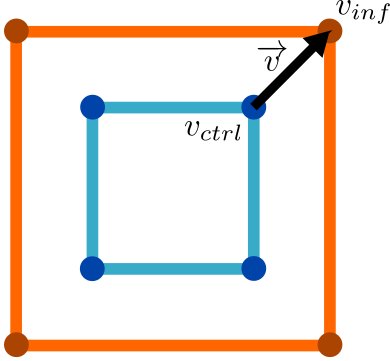
\includegraphics[scale=0.5]{chapter3-doubleCage-hierarchie-avant-pstricks}
  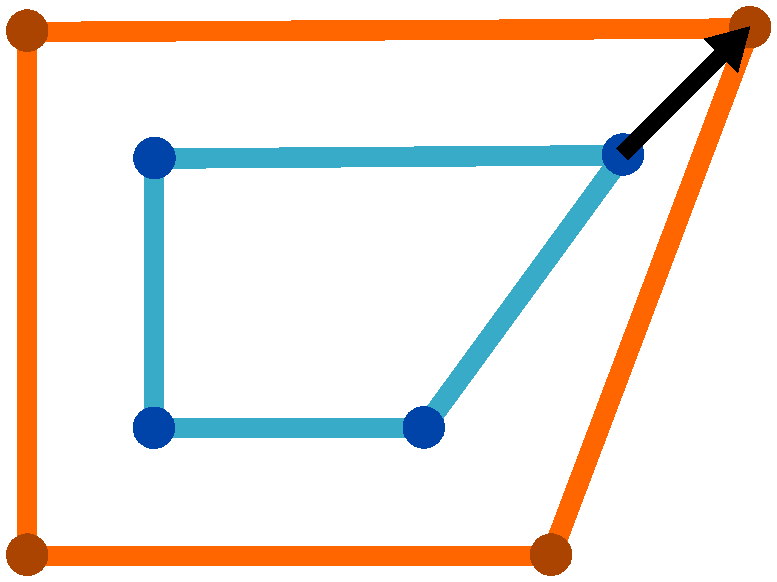
\includegraphics[scale=0.5]{chapter3-doubleCage-hierarchie-apres-pstricks}

  \caption[Association des cages de contrôle et d'influence] {Modification de
la position du sommet de la cage d'influence $v_{inf}$ associé au sommet de la
cage de contrôle déplacé $v_{ctrl}$. A gauche les cages avant déformation, à
droite les cages après déformation. En bleu la cage de contrôle, en orange la
cage d'influence et en noir le vecteur $v$.}

  \label{MelHie}
\end{center}
\end{figure}

\subsubsection{Atténuation de la déformation}

Pour l'instant, la déformation souffre toujours de problème de continuité au
niveau du bord de la cage d'influence. Pour corriger ce problème, nous allons
progressivement atténuer la déformation appliquée, en fonction de la distance
d'un point de l'espace au bord de la cage d'influence.

Pour atténuer la déformation nous avons choisi d'interpoler linéairement la
position qu'un point de l'espace avait initialement (au temps d'association)
avec la position qu'il devrait avoir avec une déformation classique:

\begin{equation}
  T_{d}(p) = \gamma p + (1-\gamma) T(p)
\end{equation}

où $p$ correspond à la position initiale du point, $T(p)$ la position que ce
point aurait après la déformation et $T_{d}(p)$ la position finale du point.

Nous avons choisi d'interpréter ce critère $\gamma$ comme représentant la
distance du point $p$ au centre de la cage d'influence. Nous utilisons les
coordonnées que nous avons déjà calculé pour chacun des points de l'espace par
rapport aux sommets de la cage d'influence. Ce choix a l'avantage de ne pas
nécessiter de réaliser des calculs supplémentaires. On établit que la distance
au bord $d_{inf}(p)$ doit être égale au produit des poids associés à chacune
des arêtes de la cage d'influence. Où le poids associé à une arête $e_i$
correspond à la somme des poids associés aux sommets incidents $v_j$ à cette
arête :

\begin{equation}
  d_{inf}(p) = f_h( \prod_{e_i \in c_{inf}} (1 - \sum_{v_j \in e_i} \lambda_j(p)))
\end{equation}

Ce calcul s'inspire de la notion de "boundary weight function" de
\cite{GPCP13}, où les auteurs utilisaient cette fonction pour évaluer la
distance d'un point à chacune des arêtes d'une cage.

La fonction $f_h(x)$, paramétrisée par $h \in ]0, 1]$, permet de lisser les
valeurs des distances des points de l'espace au bord de la cage d'influence.
Cette fonction doit satisfaire $f_h(0) = f_h'(0) = f_h'(1) = 0$, $f_h(x)=1$
pour $x \geq h$ et $f'_h(x) \geq 0$. L'idée vient du travail de \cite{GPCP13},
où ils utilisaient cette fonction pour lisser les valeurs de distance d'un
point à une arête de la cage. Les auteurs proposaient plusieurs fonctions avec
des comportements similaires, nous en avons donc gardé une arbitrairement :

\begin{equation}
  f_h(x) = \frac{1}{2} sin(\pi(\frac{x}{h} - \frac{1}{2})) + \frac{1}{2}
\end{equation}

Il faut évaluer la valeur de $h$ de manière à ce que ce paramètre représente
la différence de taille entre la cage de contrôle et la cage d'influence. On
souhaite que la déformation ne soit pas atténuée pour l'ensemble des points de
l'espace à l'intérieur de la cage de contrôle. On va donc définir une distance
$d_{min}$ telle que si la distance d'un point de l'espace au bord de la cage
d'influence est supérieure à $d_{min}$, alors la déformation de ce point ne
sera pas atténuée. $d_{min}$ correspond à la plus courte distance d'un point
de l'espace (inclus dans la cage de contrôle) au bord de la cage d'influence.
Plus précisément, il s'agit exactement de la valeur de distance du sommet de
la cage de contrôle le plus proche du bord de la cage d'influence. Il nous
suffit donc d'évaluer la valeur de distance en chacun des sommets de la cage
de contrôle par rapport au bord de la cage d'influence et de les comparer afin
de trouver la distance minimale :

\begin{equation}
  d_{min} = \min_{\forall v_{ctrl}} d_{inf}(v_{ctrl}).
\end{equation}

Plus la différence de taille entre la cage de contrôle et la cage d'influence
est grande, plus l'atténuation de la déformation est douce (Figure
\ref{MELBou}).

\begin{figure}[ht]
  \begin{center}
    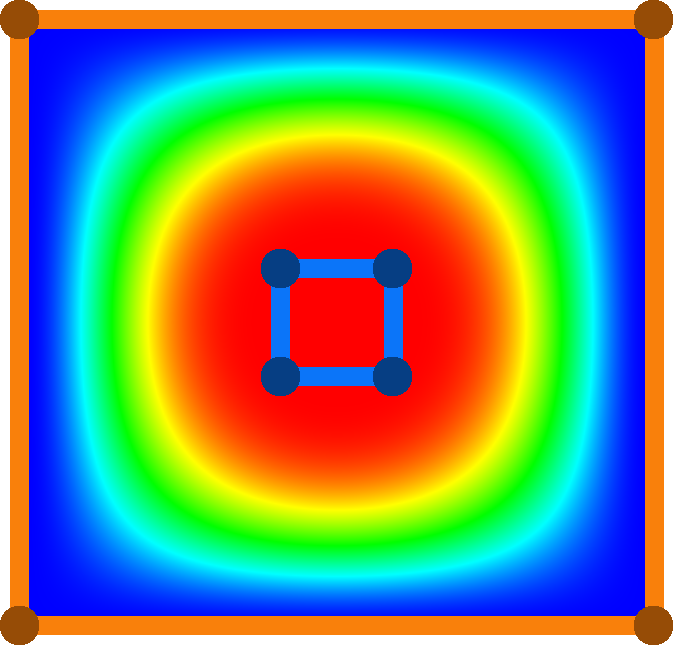
\includegraphics[scale=0.2]{BoundaryWeightFunction-Petite}
    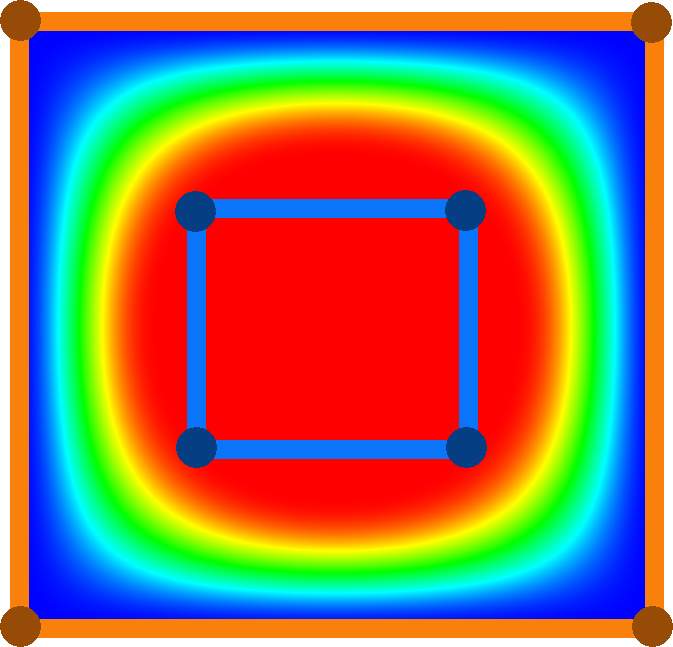
\includegraphics[scale=0.2]{BoundaryWeightFunction}
    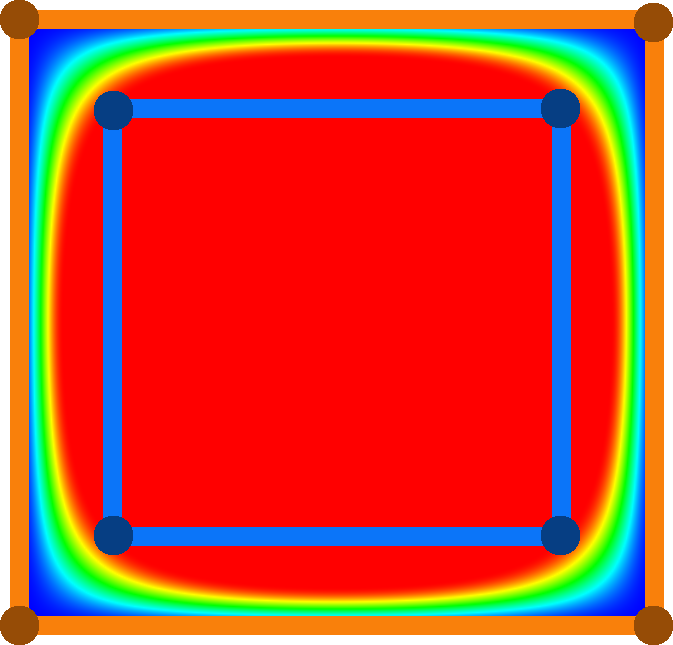
\includegraphics[scale=0.2]{BoundaryWeightFunction-Grande}

    \caption[Variation de l'atténuation de la déformation] {Variation de
l'atténuation de la déformation. La couleur varie du rouge (atténuation nulle)
au bleu (atténuation totale). De gauche à droite on peut voir la variation
pour différentes tailles de cage de contrôle.}

    \label{MELBou}
  \end{center}
\end{figure}

Ci-dessous l'algorithme représentant l'étape de déformation du modèle avec
atténuation de l'influence de la déformation: \\

\fbox{\begin{minipage}{0.9\textwidth}
  \begin{algorithm}[H]
  \KwIn{$pos$, $pos_{init}$ : tableau de tableau de réels}
  \ForEach{point de l'espace p}
  {
    $pos$[p] $\leftarrow$ [0,0]\; 
      \ForEach{sommet v de la cage d'influence c}
      {
        $pos$[p] $\leftarrow$ $pos$[p] + $\lambda_v(p)$ * $pos$[v] 
        * $d_{inf}(c, p)$\;
        $pos$[p] $\leftarrow$ $pos$[p] + $\lambda_v(p)$ * $pos_{init}$[v] 
        * (1-$d_{inf}(c, p)$)\;
      }
  }
  \caption{Déformation avec zone d'influence modifiée}
  \end{algorithm}
\end{minipage}} \\

Pour simplifier les écritures dans la suite du travail, nous nous référons à
ce nouvel outil (composé d'une cage de contrôle et d'une cage d'influence)
comme étant l'outil \textit{cage de contrôle d'influence} ou \textit{cage
coninf}.

\begin{figure}[ht]
  \begin{center}
    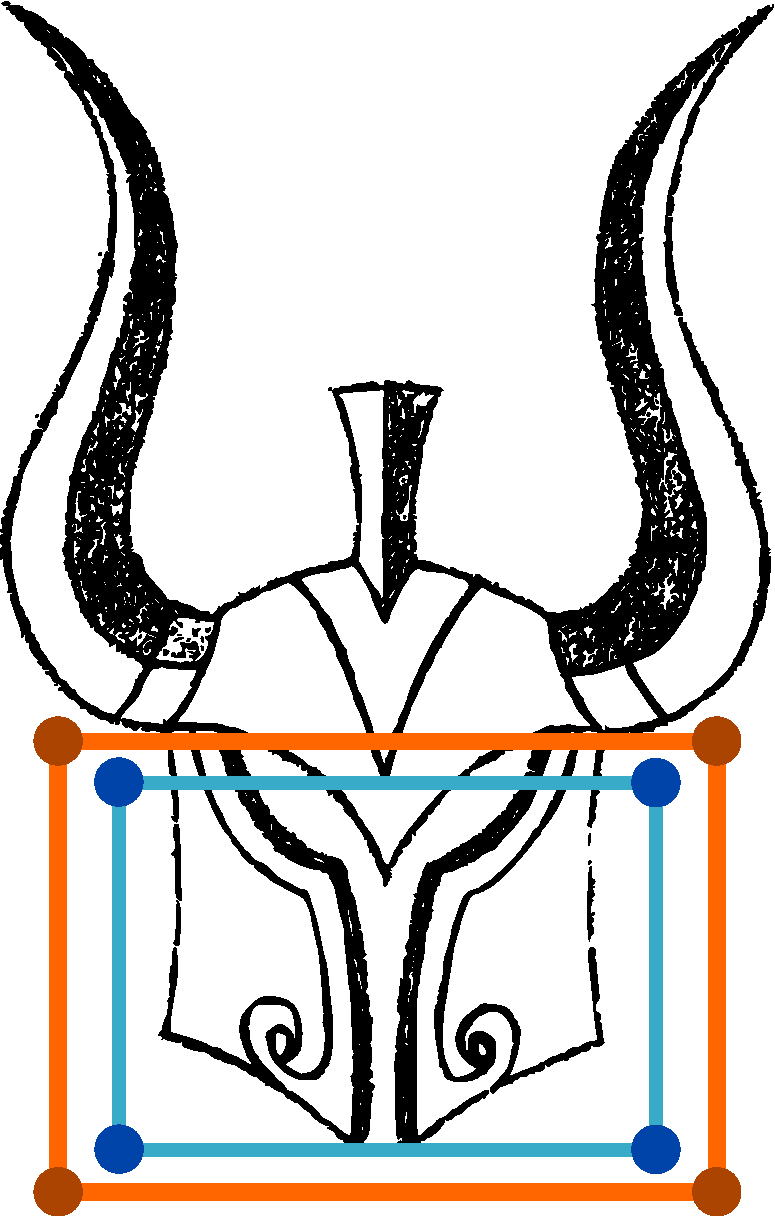
\includegraphics[scale=0.3]{Deformation-Capricorne-Avant}
    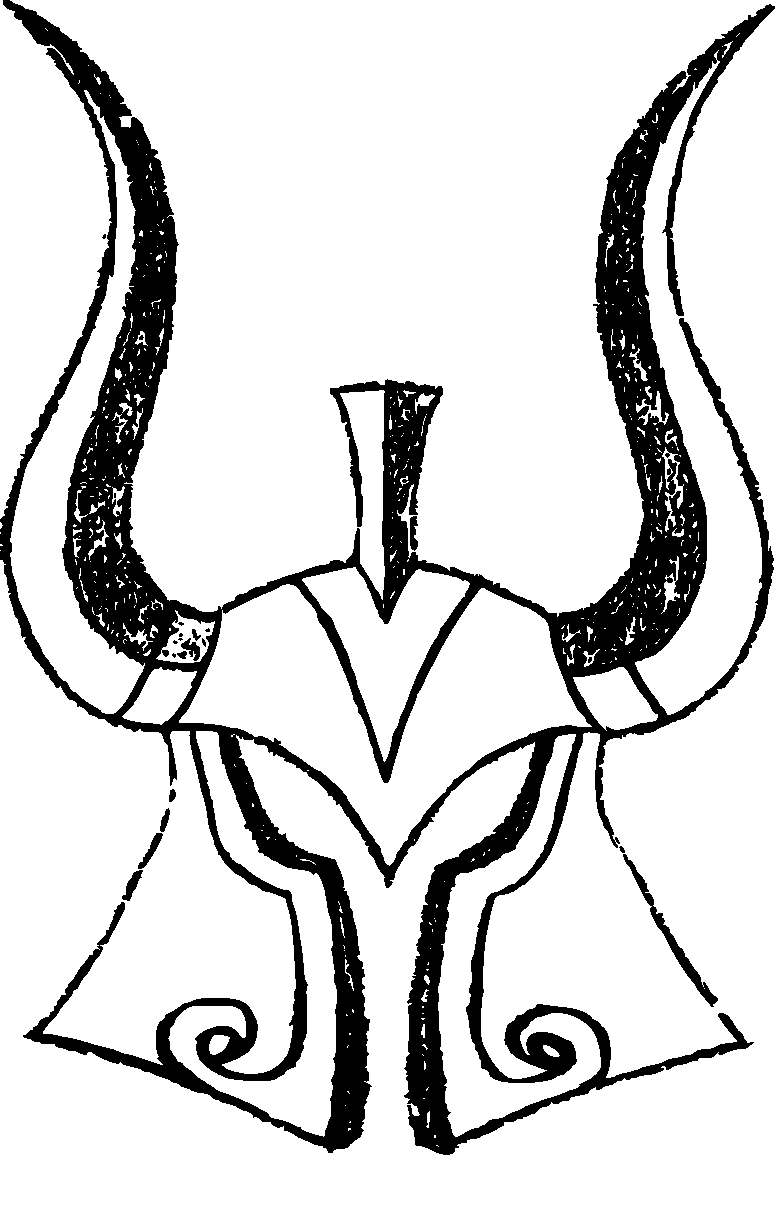
\includegraphics[scale=0.3]{Deformation-Capricorne-Apres}

    \caption[Exemple de déformation cage de contrôle d'influence] {Exemple de
déformation avec une cage de contrôle d'influence. A gauche le casque et la
cage coninf au temps d'association, à droite après modification de la position
des sommets de la cage de contrôle. On peut remarquer que la partie haute du
casque (cimier) n'a pas été modifiée par la déformation.}

  \end{center}
\end{figure}

\subsection{Combinaison des déformations}

Maintenant que nous avons établi un outil de déformation local, nous voulons
combiner plusieurs cages coninf sur un même modèle (Figure \ref{MELMC}).
L'objectif de cette partie consiste à trouver une formule de mélange
permettant la modification de la position d'un point de l'espace par rapport à
plusieurs cages coninf. De manière à ce que la déformation résultant du
mélange soit visuellement lisse.

\begin{figure}[ht]
  \begin{center}
    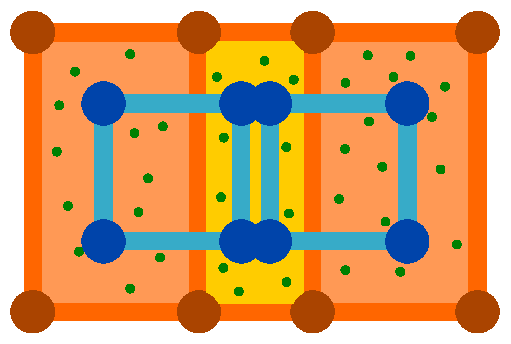
\includegraphics[scale=1]{chapter3-doubleCage-melange-pstricks}

    \caption[Mélange de cages de contrôle d'influence] {Exemple de
configuration de deux cages de contrôle d'influence se chevauchant. Les points
de l'espace (en vert) appartenant à la zone en jaune sont sous l'influence des
deux cages à la fois}

    \label{MELMC}
  \end{center}
\end{figure}

Combiner les déformations revient à établir une combinaison linéaire pondérée
de l'influence de chaque cage coninf. Pour établir la valeur du coefficient
associé à chaque cage, il faut trouver un critère permettant de classer les
cages selon l'importance de la déformation à appliquer. Le critère que nous
décidons d'envisager est celui de distance. En effet, intuitivement, plus
un point de l'espace est proche du centre d'une cage coninf, plus on aimerait
que cette cage influe sur la déformation de ce point. Autrement dit, on va
regarder la proximité d'un point de l'espace au centre de chaque cage coninf à
laquelle il appartient.

Comparer la proximité au centre d'une cage coninf revient au même que de
comparer l'éloignement au bord de la cage d'influence. Ainsi, on peut
réutiliser les valeurs de distance au bord de la cage d'influence $d_{inf}(p)$
pour connaître la proximité d'un point au centre d'une cage coninf. Ces
distances étant relatives à chaque cage, il est nécessaire de les normaliser
afin de pouvoir les comparer entre elles :

\begin{displaymath}
  D_{inf_i}(p) = \frac{d_{inf_i}(p)}{\sum_{j=0}^n d_{inf_j}(p)}, 
\end{displaymath}

où $D_{inf_i}(p)$ correspond à la distance normalisée du $p$ par rapport au
bord de la cage d'influence constituant la cage coninf $i$.

On peut maintenant définir une fonction de mélange se basant sur la proximité
d'un point de l'espace au centre des différentes cages coninf auquel il
appartient :

\begin{displaymath}
  T_{mel}(p) = \sum_{i=0}^n D_{inf_i}(p) T_{d_i}(p).
\end{displaymath}

Ci-dessous l'algorithme représentant l'étape de déformation du modèle avec le
mélange des déformations: \\

\fbox{\begin{minipage}{0.9\textwidth}
\begin{algorithm}[H]
\KwData{$sumD_{inf}$, $D_{inf}$: réel}
\KwIn{$pos$, $pos_{init}$ : tableau de tableau de réels}
\ForEach{point de l'espace p}
{
  $sumD_{inf}$ $\leftarrow$ 0\;
  \ForEach{cage d'influence c associée à p}
  {
    $sumD_{inf}$ $\leftarrow$ $sumD_{inf}$ + $d_{inf}(c, p)$\;
  }
  $pos$[p] = [0,0]\; 
  \ForEach{cage d'influence c associée à p}
  {
    $D_{inf}$ $\leftarrow$ $d_{inf}(c, p)$ / $sumD_{inf}$\;
    \ForEach{sommet v de c}
    {
      $pos$[p] $\leftarrow$ $pos$[p] + $\lambda_v(p)$ * $pos$[v] 
      * $d_{inf}(c, p)$ * $D_{inf}$\;
      $pos$[p] $\leftarrow$ $pos$[p] + $\lambda_v(p)$ * $pos_{init}$[v] 
      * (1-$d_{inf}(c, p)$) * $D_{inf}$\;
    }
  }
}
\caption{Mélange des déformations}
\end{algorithm}
\end{minipage}} \\

\begin{figure}[ht]
  \begin{center}
    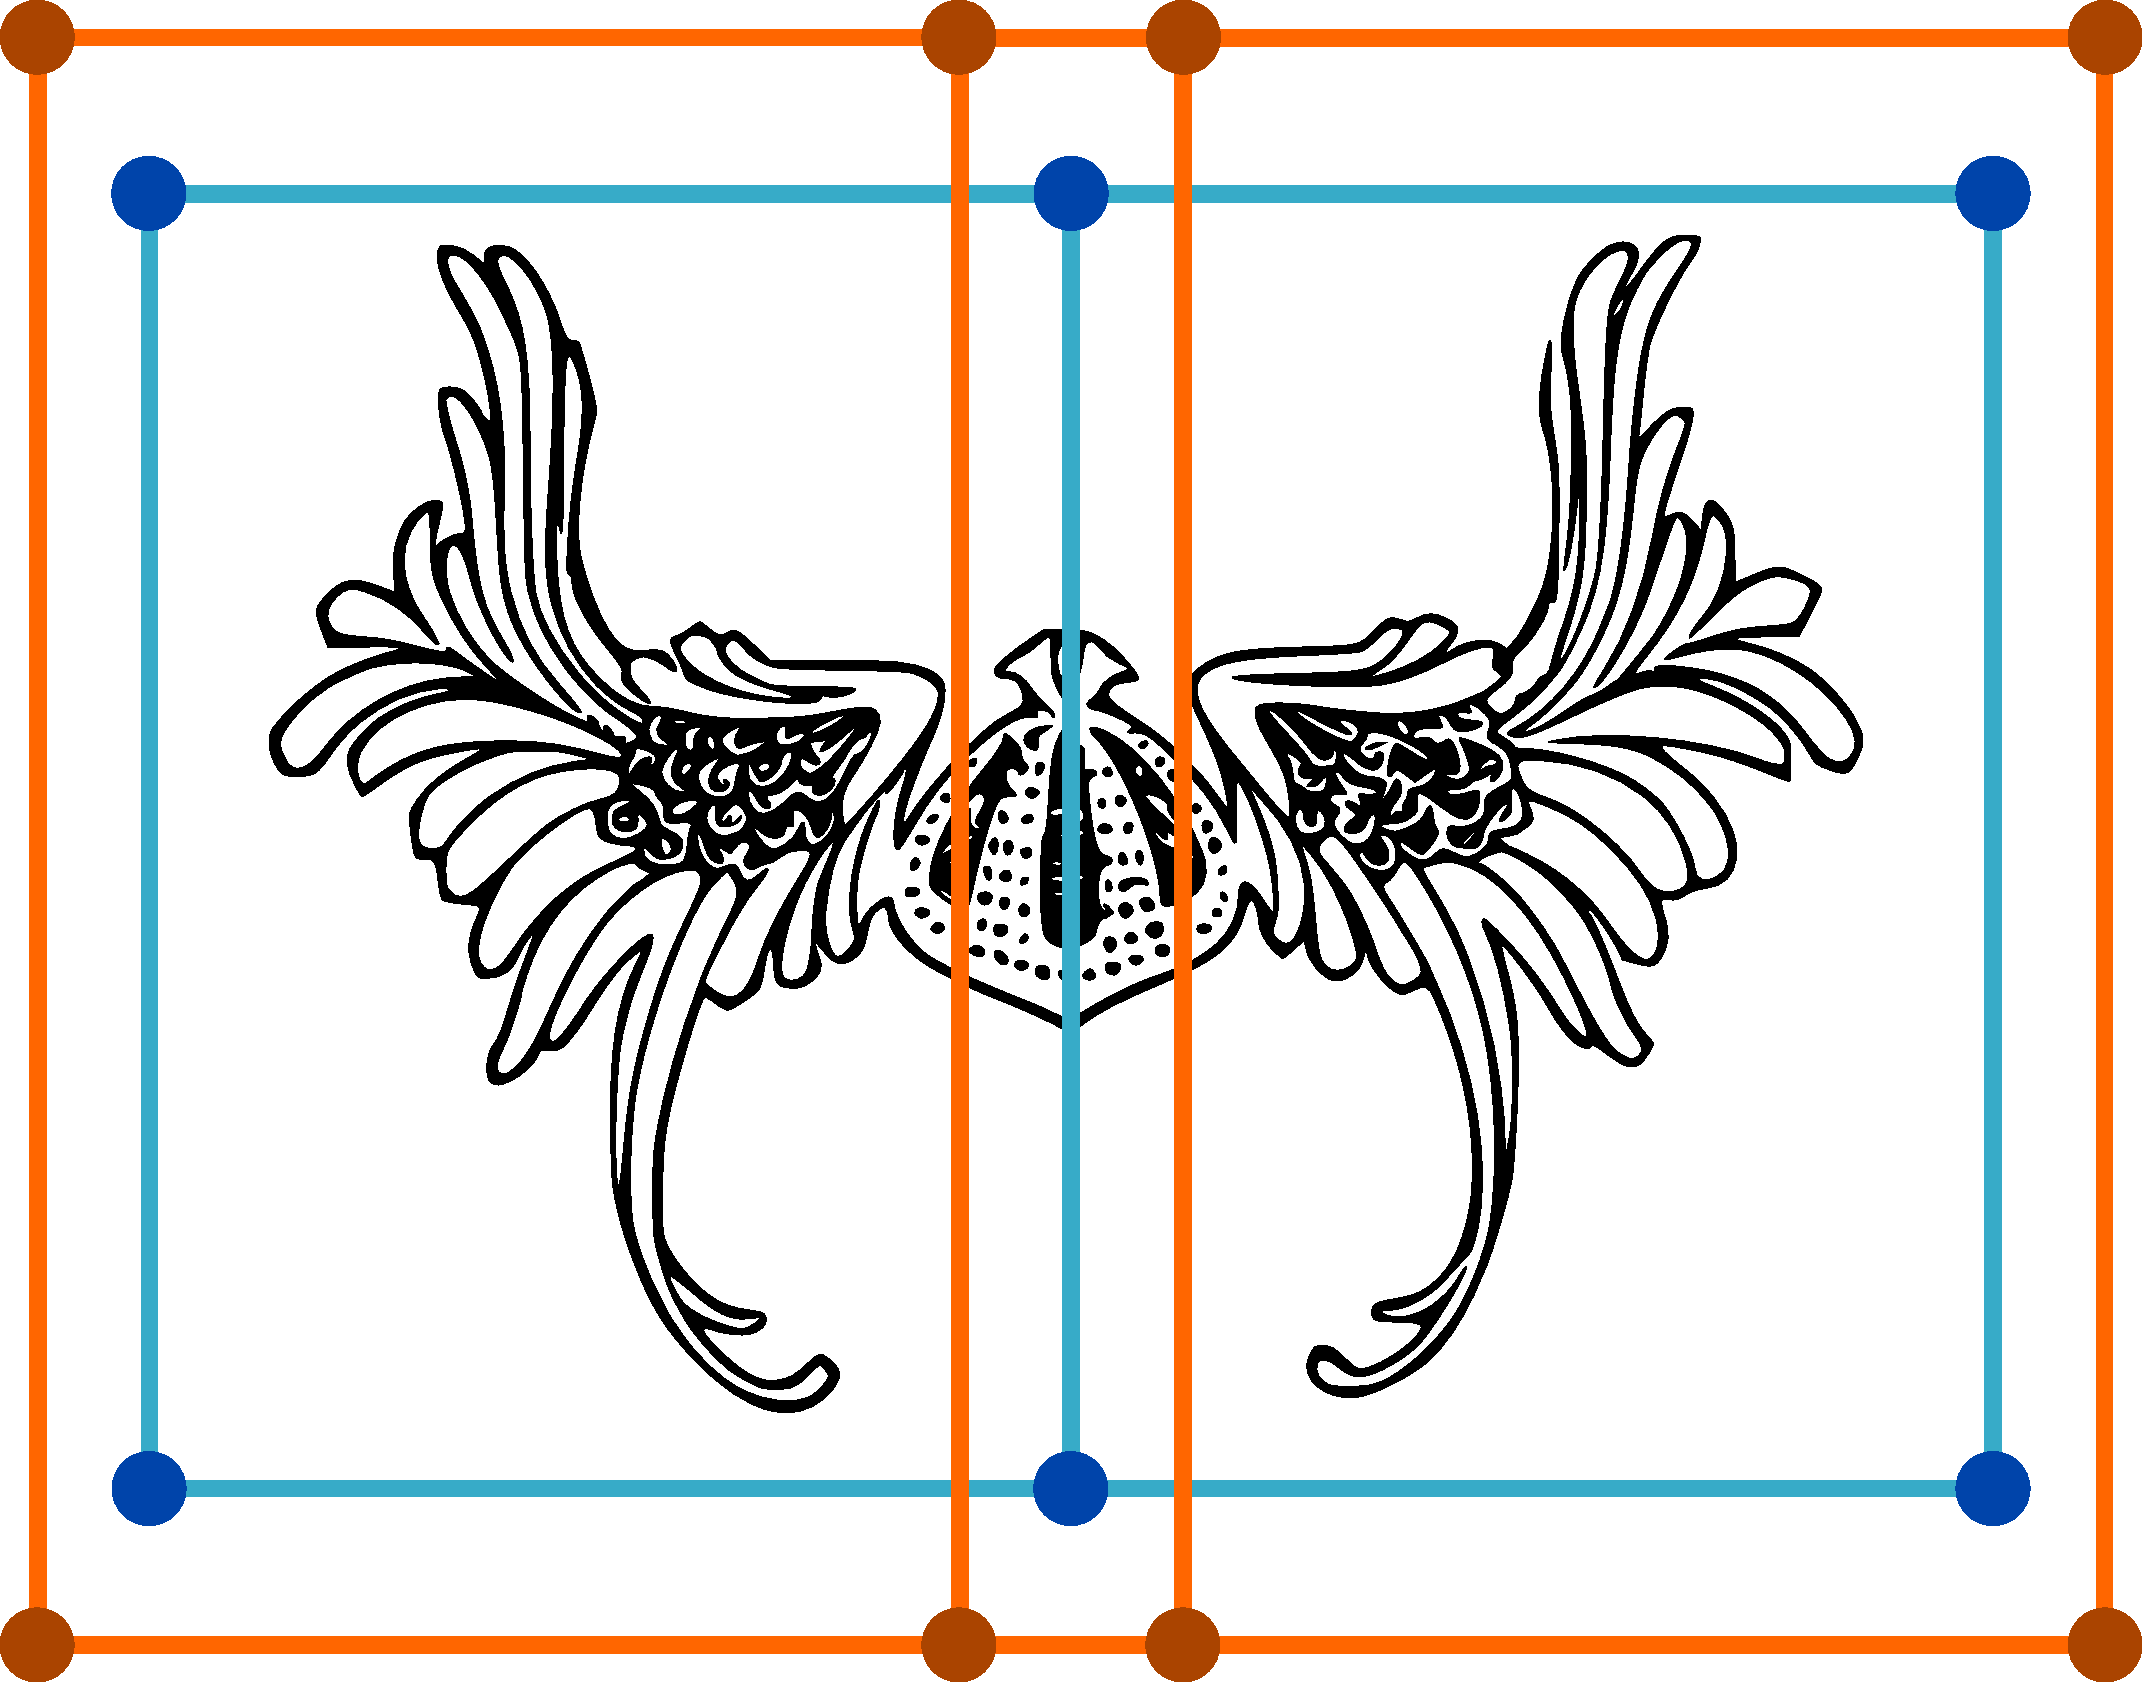
\includegraphics[scale=0.3]{Deformation-Viking-Avant}
    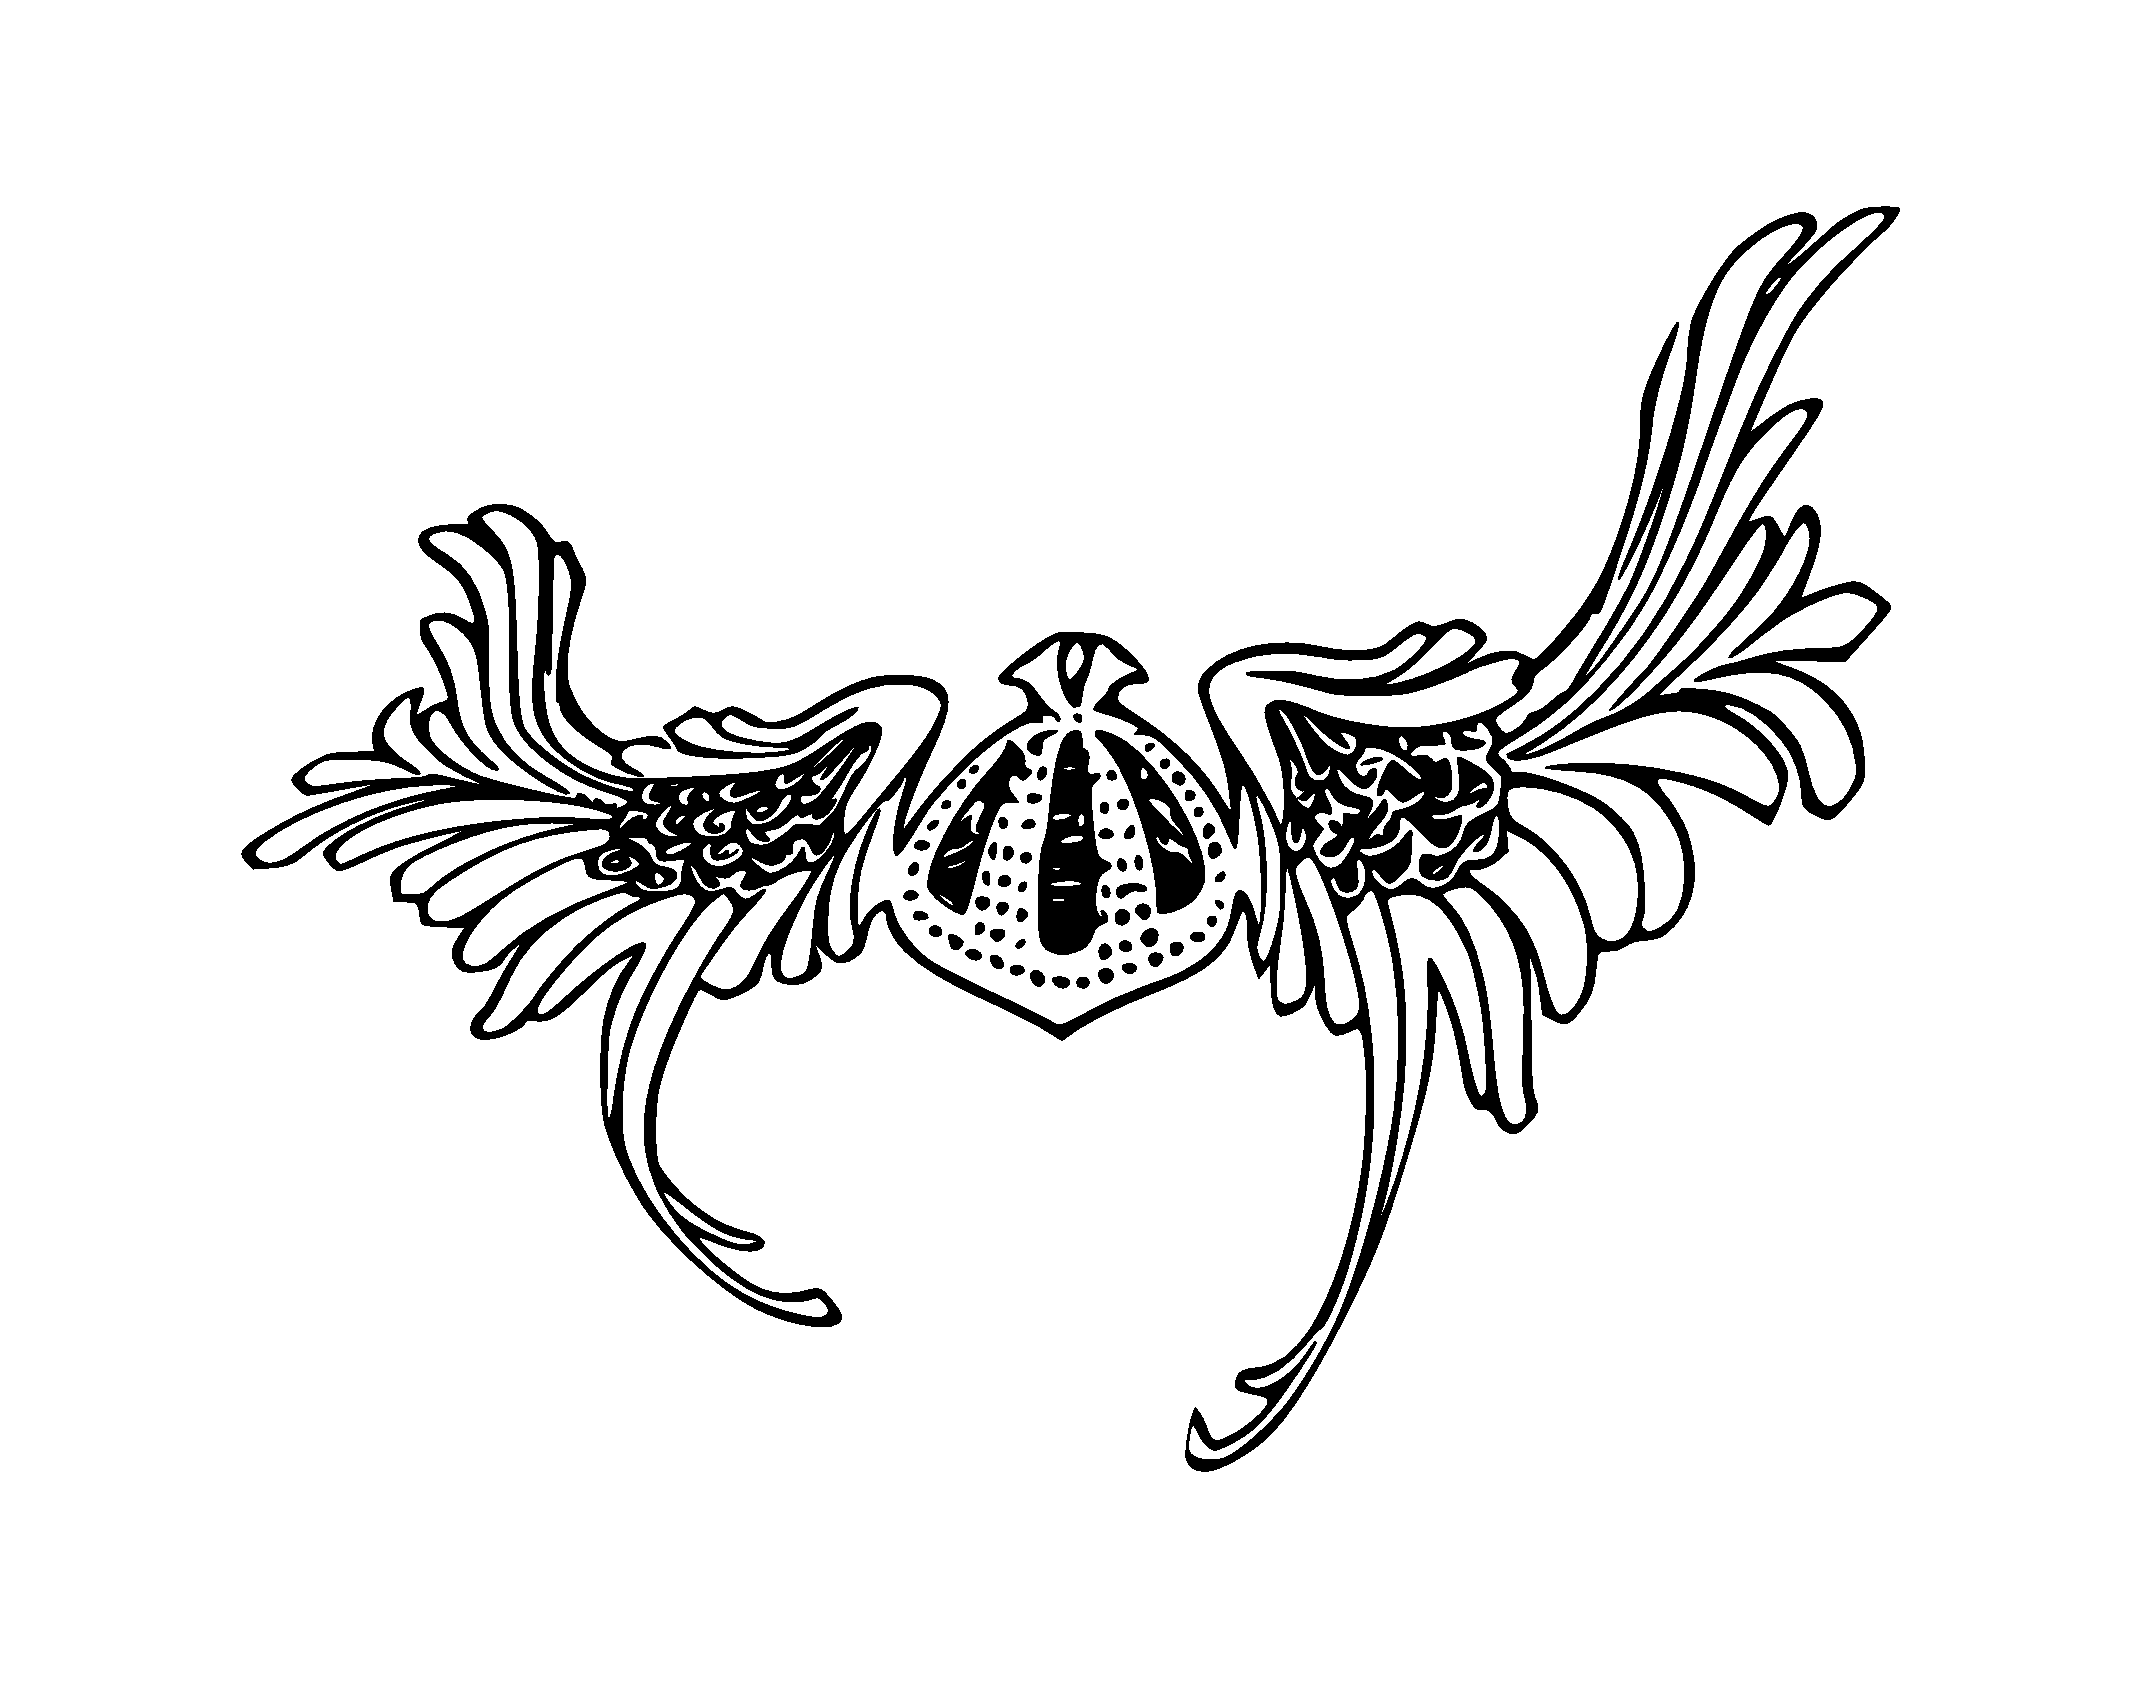
\includegraphics[scale=0.3]{Deformation-Viking-Apres}

    \caption[Exemple de déformation cage de contrôle d'influence] {Exemple de
déformation avec deux cages de contrôle d'influence (en bleu les cages de
contrôle, en orange les cages d'influence) où les cages de contrôle ont été
collées ensembles le long d'une arête commune. A gauche le casque avant
déformation, à droite après modification de la position des sommets des deux
cages de contrôle.}

  \end{center}
\end{figure}

